%   % !TEX root = ../../VIII,3_Rahmen-TeX_8-1.tex
%
%
%   Band VIII, 3 N.~??A37
%   Signatur/Tex-Datei: LH_37_05_001
%   RK-Nr. 60273
%   Überschrift: De motu
%   Modul: Mechanik / Elastizität
%   Datierung: [Ende 1674 bis Ende 1677 (?)]
%   WZ: (keins)
%   SZ: (keins)
%   Bilddateien (PDF): LH_37_05_001_d1; LH_37_05_001_d2; LH_37_05_001_d3; LH_37_05_001_d4; LH_37_05_001_d5; LH_37_05_001_d6 (insgesamt: sechs)
%
%
\selectlanguage{ngerman}%
\frenchspacing%
%
\begin{ledgroupsized}[r]{120mm}
\footnotesize
\pstart
\noindent\textbf{Überlieferung:}
\pend
\end{ledgroupsized}
\begin{ledgroupsized}[r]{114mm}
\footnotesize
\pstart
\parindent -6mm
\makebox[6mm][l]{\textit{L}}%
Konzept: LH~XXXVII~5 Bl.~1.
Ein Blatt 2\textsuperscript{o};
rechter Rand von Bl.~1~r\textsuperscript{o} beschnitten mit geringfügigem Textverlust;
Papiererhaltungsmaßnahmen.
Eineinhalb Seiten;
untere Hälfte von Bl.~1~v\textsuperscript{o} leer.
Am rechten Rand von Bl.~1~v\textsuperscript{o} Reste eines Diagramms (mit den ausgewiesenen Punkten \textit{R}, \textit{Q} und \textit{T}), welches offenbar auf einem ursprünglich verbundenen, nicht weiter bekannten Blatt vorlag.
\pend
\end{ledgroupsized}
%
%
\vspace{5mm}
\begin{ledgroup}
\footnotesize 
\pstart
\noindent\textbf{Datierungsgründe:}
Im vorliegenden Entwurf N.~4 % \textit{De motu} 
nimmt Leibniz eine stoßtheoretische Beobachtung zum Anlass, Überlegungen über die Festigkeit und das elastische Verhalten der Körper anzustellen.
Gleich zu Beginn erwähnt er die 1669 veröffentlichten Aufsätze von J.~Wallis, C. Wren und C. Huygens über die Gesetze des zentralen Stoßes, wobei er betont, dass diese Gesetze nicht von der \glqq absoluten Natur der Bewegung\grqq\ ableitbar seien (S.~\refpassage{LH_37_05_001r_regulaemotus_bgsf-1}{LH_37_05_001r_regulaemotus_bgsf-2}).%
\protect\index{Namensregister}{\textso{Huygens} (Hugenius, Ugenius, Hugens, Huguens), Christiaan 1629\textendash1695}%
\protect\index{Namensregister}{\textso{Wallis} (Wallisius), John 1616\textendash1703}%
\protect\index{Namensregister}{\textso{Wren} (Wrennus), Christopher 1632\textendash1723}
Diese Erwähnung ist Grund für die Annahme, dass N.~4 noch in den Siebziger Jahren entstand, als Leibniz an der methodologischen Unterscheidung zwischen \glqq abstrakter\grqq\ und \glqq konkreter\grqq\ Betrachtung der Bewegung, wie er sie 1671 in den beiden \textit{Theoriae motus} getroffen hatte, noch festhielt.
Eine Bemerkung im Schlussteil von N.~4 (\textit{Casus ut duo corpora dura in vacuo concurrant, est inanis atque alienus a natura rerum}, S.~\refpassage{LH_37_05_001v_casusinanis_rltn-1}{LH_37_05_001v_casusinanis_rltn-2}) zeigt jedoch, dass Leibniz von der genannten methodologischen Unterscheidung bereits Abstand zu nehmen begonnen hatte.
Demnach dürfte N.~4 nicht vor den späteren Pariser\protect\index{Ortsregister}{Paris} Jahren entstanden sein.
Diese Schlussfolgerung wird dadurch bekräftigt, dass die stoßtheoretische Beobachtung, an die N.~4 eingangs anknüpft (S.~\refpassage{LH_37_05_001r_Anfang_jhdagiacuz-1}{LH_37_05_001r_Anfang_jhdagiacuz-2}), stark einem Beispiel ähnelt, das Leibniz in seinen auf die letzten Monate 1674 datierbaren Auszügen aus E.~Mariottes Abhandlung \textit{De la percussion}\cite{00311} (1673) 
anführt und erörtert (\textit{LSB} VIII,~2 N.~50, S.~441.16\textendash442.9).\cite{01292}%
\protect\index{Namensregister}{\textso{Mariotte}, Edme, Seigneur de Chazeuil ca. 1620\textendash1684}
Ende 1674 dürfte somit als Terminus post quem der Datierung von N.~4 gelten.
\pend%
\pstart%
% (2) N.~??A37 beruft sich auf \textit{illud principium, Conatum naturae semper irresistibilem esse}. Entspricht dies etwa der \textit{Regle generale de la nature: La même quantité d'effort pour un meême mouuement, demeure toujours} (\textit{LSB} VIII,~2 N.~34\textsubscript{1}, S.~290.17\textendash18) ??
Ausschlaggebend für die Bestimmung eines Terminus ante quem könnte die im Text verwendete Begrifflichkeit sein.
Bei der Erörterung eines auf das Diagramm \lbrack\textit{Fig.~2}\rbrack\ bezogenen Beispiels (S.~\refpassage{LH_37_05_001r_nopeusvoimana_msdhg-1}{LH_37_05_001r_nopeusvoimana_msdhg-2}) setzt Leibniz die Geschwindigkeit (\textit{celeritas}) eines stoßenden Körpers noch seiner Kraft (\textit{vis}) gleich.
Rührt diese Wortwahl nicht von bloßer Ungenauigkeit her, so ist sie als Zeichen dafür zu deuten, dass der Entwurf N.~4 vor Januar 1678 entstanden sein muss.
\pend 
\end{ledgroup}
\selectlanguage{latin}%
\frenchspacing%
%
%
\count\Bfootins=1200
\count\Afootins=1200
\count\Cfootins=1200
%\newpage%
 \vspace{8mm}
\pstart%
\normalsize%
\noindent%
\lbrack1~r\textsuperscript{o}\rbrack\
\pend%
\vspace{-0.5em}
%
\pstart%
\centering%
De Motu
\pend%
\vspace{0.5em}
%
\pstart%
\noindent%
\edtext{Certum\edlabel{LH_37_05_001r_Anfang_jhdagiacuz-1} est
%
\edtext{pilam\protect\index{Sachverzeichnis}{pila propulsa} \textit{A}}{%
\lemma{pilam \textit{A}}\Cfootnote{%
Siehe das Diagramm \lbrack\textit{Fig.~1}\rbrack\ auf S.~\pageref{LH_37_05_001r_Fig.1}.}}
%
in
%
\edtext{aliam}{%
\lemma{aliam}\Bfootnote{%
\textit{erg.~L}}}
%
aequalem et similem \textit{B} tarde propulsam,
continuare motum\protect\index{Sachverzeichnis}{motus pilae}
eamque secum abripere,
at si celeriter impingat,\protect\index{Sachverzeichnis}{pila impacta}
%
\edtext{tunc propellere \textit{B},}{%
\lemma{tunc}\Bfootnote{%
\textit{(1)}~propulsa \textit{B},
\textit{(2)}~propellere \textit{B},%
~\textit{L}}}
%
et in ejus loco quiete consistere.%
\edlabel{LH_37_05_001r_Anfang_jhdagiacuz-2}%
}{\lemma{Certum \lbrack...\rbrack\ consistere}\Cfootnote{%
Ein ähnliches Beispiel erörtert Leibniz in einer Bemerkung zu seinen Auszügen aus E.~\textsc{Mariotte}, \textit{Traité de la percussion}, Paris 1674\cite{00311} (\textit{LSB} VIII,~2 N.~50, S.~441.16\textendash442.9).\cite{01292}}}
%
Hinc colligitur\lbrack:\rbrack\
%
\edlabel{LH_37_05_001r_regulaemotus_bgsf-1}%
\edtext{regulas motuum\protect\index{Sachverzeichnis}{regula motus}
quae a doctissim\textlangle is\textrangle\ viris\protect\index{Sachverzeichnis}{vir doctus}%
\protect\index{Namensregister}{\textso{Wallis} (Wallisius), John 1616-1703}%
\protect\index{Namensregister}{\textso{Wren} (Wrennus), Christopher 1632-1723}%
\protect\index{Namensregister}{\textso{Huygens} (Hugenius, Ugenius, Hugens, Huguens), Christiaan 1629-1695}
in Gallicis Anglicisque diariis%
\protect\index{Sachverzeichnis}{diarius Gallicus}\protect\index{Sachverzeichnis}{diarius Anglicus}
sunt publicatae}{%
\lemma{regulas \lbrack...\rbrack\ publicatae}\Cfootnote{%
Siehe
\textsc{J.~Wallis}, \cite{01065}\glqq A summary account \lbrack...\rbrack\ of the general laws of motion\grqq, \textit{PT} III (1668), S.~864\textendash866; %
\textsc{C.~Wren}, \cite{01066}\glqq Theory concerning the same subject\grqq, \textit{PT} III (1668), S.~867\,f.; %
\textsc{C.~Huygens}, \cite{00529}\glqq Règles du mouvement dans la rencontre des corps\grqq, \textit{JS}, 18. März 1669, S.~22\textendash24 %
(\cite{00113}\textit{HO} VI, S.~383\textendash386); %
\textsc{Ders.}, \cite{01067}\glqq A summary account of the laws of motion\grqq, \textit{PT} IV (1669), S.~925\textendash928 %
(\cite{00113}\textit{HO} VI, S. 429\textendash433).}}
%
ex particularibus quibusdam
%
\edtext{causis\protect\index{Sachverzeichnis}{causa particularis}
et subjecti\protect\index{Sachverzeichnis}{conditio subjecti} conditio\textlangle nibus\textrangle\
oriri}{%
\lemma{causis}\Bfootnote{%
\textit{(1)}~oriri
\textit{(2)}~et subjecti conditio\textlangle nibus\textrangle\ oriri%
~\textit{L}}}%
\lbrack,\rbrack\
%
non ex absoluta motus natura,\protect\index{Sachverzeichnis}{natura motus absoluta}
neque enim alioquin motus celer\protect\index{Sachverzeichnis}{motus celer}
a parvo\protect\index{Sachverzeichnis}{motus parvus} differret.%
\edlabel{LH_37_05_001r_regulaemotus_bgsf-2}
\pend%
\count\Bfootins=1000
\count\Afootins=1200
\count\Cfootins=1000
%
\pstart%
Suspicor autem rationem esse,
quod ictui celeri\protect\index{Sachverzeichnis}{ictus celeris}
%
\edtext{cedit corporum}{\lemma{cedit}\Bfootnote{%
\textit{(1)}~corporis
\textit{(2)}~corporum%
~\textit{L}}}
%
firmitas\protect\index{Sachverzeichnis}{firmitas corporis}
et perinde habentur
ac si mollia essent,\protect\index{Sachverzeichnis}{corpus molle}
ipsa vero postea se restituunt,\protect\index{Sachverzeichnis}{corpus se restituens}
unde si tanta sit celeritas,\protect\index{Sachverzeichnis}{celeritas ictus}
ut flexio\protect\index{Sachverzeichnis}{flexio corporis}
atque transformatio\protect\index{Sachverzeichnis}{transformatio corporis} contingat
ante omnem corporum promotionem,\protect\index{Sachverzeichnis}{promotio corporis}
perfecte locum habebunt regulae\protect\index{Sachverzeichnis}{regula motus}
a clarissimis viris\protect\index{Sachverzeichnis}{vir clarus} allatae.
\pend%
\pstart%
Idem experimento\protect\index{Sachverzeichnis}{experimentum circuli ferrei}
circuli ferrei\protect\index{Sachverzeichnis}{circulus ferreus} confirmatur,
qui fortiter percussus prius inflectitur quam totus cedat,
contrarium evenit, si debiliter impellatur.
\pend%
%
\pstart%
Explicandum\edlabel{LH_37_05_001r_nopeusvoimana_msdhg-1} tamen\setline{11} superest,
cur potius cedat hoc casu pars quam totum,
quod tali similitudine\protect\index{Sachverzeichnis}{similitudo} explicabo:
sit vas \textit{B}
%
\edtext{suspensum\protect\index{Sachverzeichnis}{vas suspensum}}{%
\lemma{suspensum}\Bfootnote{%
\textit{erg.~L}}}
%
plenum\protect\index{Sachverzeichnis}{vas plenum materia cedente}
materia cedente\protect\index{Sachverzeichnis}{materia cedens}
ut pice\protect\index{Sachverzeichnis}{pix} \textit{C},
in quam ingredi
%
\edtext{possit a latere corpus \textit{A}; si}{%
\lemma{possit}\Bfootnote{%
\hspace{-0,5mm}\textbar~a latere \textit{erg.}~%
\textbar\ corpus \textit{A};
\textbar~ajo \textit{gestr.}~%
\textbar\ si%
~\textit{L}}}
%
major sit celeritas\protect\index{Sachverzeichnis}{celeritas corporis ingredientis}
quam resistentia picis,\protect\index{Sachverzeichnis}{resistentia picis}
cedet pix\protect\index{Sachverzeichnis}{pix} potius
%
\edtext{quam ut vas\protect\index{Sachverzeichnis}{vas suspensum}}{%
\lemma{quam}\Bfootnote{%
\textit{(1)}~vas
\textit{(2)}~ut vas%
~\textit{L}}}
%
moveatur,
imo vas impetum\protect\index{Sachverzeichnis}{impetus} ne sensurum esset quidem,
si sensu\protect\index{Sachverzeichnis}{sensus} praeditum esset.
Si vero major esset resistentia picis,\protect\index{Sachverzeichnis}{resistentia picis}
quam vis corporis\protect\index{Sachverzeichnis}{vis corporis} \textit{A},
vas\protect\index{Sachverzeichnis}{vas suspensum} totum cederet.%
\edlabel{LH_37_05_001r_nopeusvoimana_msdhg-2}
\pend%
%\vspace{1em}
\pstart%
Alia\edlabel{LH_37_05_001r_deduabustabulis_hgx-1} utor similitudine,\protect\index{Sachverzeichnis}{similitudo}
sint duae
%
\edtext{tabulae planae\protect\index{Sachverzeichnis}{tabula plana}
compositae,\protect\index{Sachverzeichnis}{tabulae compositae}}{%
\lemma{tabulae}\Bfootnote{%
\textit{(1)}~congruentes
\textit{(2)}~planae compositae,%
~\textit{L}}}
%
ne facile
%
\edtext{\lbrack quidem\rbrack}{%
\lemma{quidem}\Bfootnote{\textit{erg. Hrsg.}}}
%
separari
%
\edtext{possint, inferior}{%
\lemma{possint,}\Bfootnote{%
\textit{(1)}~stentque erectae, ita
\textit{(2)}~inferior%
~\textit{L}}}
%
\textit{CD} superior
%
\edtext{\textit{AB}, globulus}{%
\lemma{\textit{AB},}\Bfootnote{%
\textit{(1)}~globus
\textit{(2)}~globulus%
~\textit{L}}}
%
\textit{E} sursum tendens impingat in supe-
\pend
\setline{1}
\pstart \vspace{1em} %\noindent
\hspace{5mm}
\begin{minipage}[t]{0.33\textwidth}
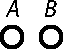
\includegraphics[width=0.2\textwidth]{gesamttex/edit_VIII,3/images/LH_37_05_001_d1.pdf}
\end{minipage}
%\hspace{4,3mm}
\begin{minipage}[t]{0.33\textwidth}
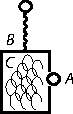
\includegraphics[width=0.39\textwidth]{gesamttex/edit_VIII,3/images/LH_37_05_001_d2.pdf}
\end{minipage}
%\hspace{4,3mm}
\begin{minipage}[t]{0.33\textwidth}
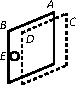
\includegraphics[width=0.5\textwidth]{gesamttex/edit_VIII,3/images/LH_37_05_001_d3.pdf}
\end{minipage}
\newline
\\
%\vspace{2em}
\hspace*{11mm} [\textit{Fig. 1}]\label{LH_37_05_001r_Fig.1}\hspace{34mm} [\textit{Fig. 2}] \label{LH_37_05_001r_Fig.2}\hspace{36mm} [\textit{Fig. 3}] \label{LH_37_05_001r_Fig.3}
\pend
%\vspace{1em}
%\newpage
%
%%
%%  \newpage% 
%  \vspace{2.5em}%	% Diagramm Fig.~1
%  \centerline{\hspace*{-85mm}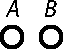
\includegraphics[width=0.072\textwidth]{gesamttex/edit_VIII,3/images/LH_37_05_001_d1.pdf}}%
%  \vspace{0.5em}
%  \centerline{\hspace*{-85mm}\lbrack\textit{Fig.~1}\rbrack}%
%  \label{LH_37_05_001r_Fig.1}%
%%  \vspace{1.5em}%
%%  \newpage%
%%
%%  \newpage% 
%  \vspace{-5.0em}%	% Diagramm Fig.~2
%  \centerline{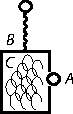
\includegraphics[width=0.13\textwidth]{gesamttex/edit_VIII,3/images/LH_37_05_001_d2.pdf}}%
%  \vspace{0.5em}
%  \centerline{\lbrack\textit{Fig.~2}\rbrack}%
%  \label{LH_37_05_001r_Fig.2}%
%%  \vspace{1.5em}%
%%  \newpage%
%%
%%  \newpage% 
%  \vspace{-9.5em}%	% Diagramm Fig.~3
%  \centerline{\hspace*{85mm}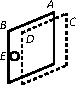
\includegraphics[width=0.18\textwidth]{gesamttex/edit_VIII,3/images/LH_37_05_001_d3.pdf}}%
%  \vspace{0.5em}
%  \centerline{\hspace*{85mm}\lbrack\textit{Fig.~3}\rbrack}%
%  \label{LH_37_05_001r_Fig.3}%
%%  \vspace{1.5em}%
 % \newpage%
%
%
\newpage
\pstart
\noindent
riorem, ajo si minor sit vis globi,\protect\index{Sachverzeichnis}{vis globi}
quam planorum connexio,\protect\index{Sachverzeichnis}{connexio planorum}
sublaturum esse tabulam utramque,%
\protect\index{Sachverzeichnis}{tabula plana}\protect\index{Sachverzeichnis}{tabulae compositae}
sin major
futurum esse,
ut inferiore ne sentiente quidem ictum\protect\index{Sachverzeichnis}{ictus globi}
superior sola tollatur.
\pend%
\count\Bfootins=1200
\count\Afootins=1200
\count\Cfootins=1200
%
\pstart%
Idem experimento\protect\index{Sachverzeichnis}{experimentum baculi vitris superpositi}
constat cum
%
\edtext{\edlabel{LH_37_05_001r_baculusvitroimpositus-1}baculus\protect\index{Sachverzeichnis}{baculus vitris superpositus}
super duobus vitris\protect\index{Sachverzeichnis}{vitrum} frangitur,}{%
\lemma{baculus \lbrack...\rbrack\ frangitur}\Cfootnote{%
Ähnliches Beispiel in N.~12\textsubscript{1}, S.~\refpassage{LH_37_01_018v_baculusvitroimpositus-1}{LH_37_01_018v_baculusvitroimpositus-2}.
Siehe zudem H.~\textsc{Fabri}, \textit{Physica}, tract.~II, lib.~V, prop.~46 (Bd.~I, Lyon 1669, S.~581b).\cite{00044}
Leibniz hat diese Stelle exzerpiert (\textit{LSB} VIII,~2 N.~55, S.~515.25\textendash27).\cite{01234}}}
%
nam si satis fortis sit ictus\protect\index{Sachverzeichnis}{ictus fortis}
baculus rumpetur,\protect\index{Sachverzeichnis}{baculus ruptus}
vitra\protect\index{Sachverzeichnis}{vitrum} non sentient
%
\edtext{ictum.\edlabel{LH_37_05_001r_baculusvitroimpositus-2}\protect\index{Sachverzeichnis}{ictus rumpens}
Ratio est,}{%
\lemma{ictum.}\Bfootnote{%
\textit{(1)}~Et ratio est,
\textit{(2)}~Ratio est,%
~\textit{L}}}
%
quia tabula inferior non impellitur,
nisi quando superior moveri non potest,
quin ipsa moveatur,
nunc vero superior omnino moveri potest,
ipsa non mota.%
\protect\index{Sachverzeichnis}{tabula plana}\protect\index{Sachverzeichnis}{tabulae compositae}
Ita si funis\protect\index{Sachverzeichnis}{funis tensus} tensus sit
secari poterit celeri ictu,\protect\index{Sachverzeichnis}{ictus celeris}
%
% \edtext{}{%
% \lemma{ita}\Bfootnote{%
% \textit{(1)}~ut
% \textit{(2)}~ut%
% ~\textit{L}}}
%
ita ut ea
quibus ab utraque vel alterutra parte annexus est
non evertantur.\edlabel{LH_37_05_001r_deduabustabulis_hgx-2}
\pend 
%
\pstart
Ut autem rem omnem ad experimentum pure mechanicum reducamus,%
\protect\index{Sachverzeichnis}{experimentum mechanicum}
sic agemus.
%
\edtext{}{%
{\xxref{LH_37_05_001r_baculusABD-1}{LH_37_05_001r_baculusABD-2}}%
{\lemma{Sit baculus \textit{ABD}}\Cfootnote{%
Siehe das Diagramm \lbrack\textit{Fig.~4}\rbrack.}}}%
%
\edlabel{LH_37_05_001r_baculusABD-1}%
Sit baculus\protect\index{Sachverzeichnis}{baculus mobilis}
%
\edtext{\textit{ABD}\edlabel{LH_37_05_001r_baculusABD-2}
mobilis circa \textit{A}, et pars ejus}{%
\lemma{\textit{ABD}}\Bfootnote{%
\textit{(1)}~cujus
\textit{(2)}~mobilis circa \textit{A}, et pars ejus%
~\textit{L}}}
%
\textit{BD} mobilis circa \textit{B}
si \textit{AB} immota maneat.
Ponamus autem non posse moveri \textit{BD} circa \textit{B}
quin elevet pondus \textit{E},%
\protect\index{Sachverzeichnis}{pondus elevandum}
neque \textit{AD} circa \textit{A}
quin elevet pondus \textit{F}.
Sit autem pondus
%
\edtext{\lbrack\textit{E}\rbrack}{%
\lemma{\textit{B}}\Bfootnote{%
\textit{L~ändert Hrsg.}}}
%
longe majus quam pondus \textit{F}.
Jam aliud pondus \textit{C} applicetur in \textit{D}.%
\protect\index{Sachverzeichnis}{pondus elevandum}
Hoc si tale sit
ut majorem
(\protect\vphantom)%
habita distantiae a centro%
\protect\index{Sachverzeichnis}{distantia a centro}
ratione%
\protect\vphantom()
vim\protect\index{Sachverzeichnis}{vis ponderis} habeat
quam pondus \textit{F},\protect\index{Sachverzeichnis}{pondus elevandum}
minorem vero quam \textit{E},
totus baculus\protect\index{Sachverzeichnis}{baculus mobilis} movebitur circa \textit{A}. Quod
%
\edtext{si majorem vim\protect\index{Sachverzeichnis}{vis ponderis}
habeat quam \textit{F} et majorem}{%
\lemma{si}\Bfootnote{%
\hspace{-0,5mm}majorem
\textbar~tantum \textit{gestr.}~\textbar\ vim habeat quam \textit{F}
\textit{(1)}~pariter
\textit{(2)}~et majorem%
~\textit{L}}}
%
etiam quam \textit{E}
tunc baculus movebitur\protect\index{Sachverzeichnis}{baculus mobilis}
\pend
%  \newpage% 
  \vspace{1.0em}%	% Diagramm Fig.~4
  \centerline{\hspace*{-86mm}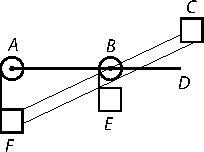
\includegraphics[width=0.29\textwidth]{gesamttex/edit_VIII,3/images/LH_37_05_001_d4.pdf}}%
  \vspace{0.0em}
  \centerline{\hspace*{-86mm}\lbrack\textit{Fig.~4}\rbrack}%
  \label{LH_37_05_001r_Fig.4}%
%  \vspace{1.5em}%
%  \newpage%
%
%  \newpage% 
  \vspace{-9.5em}%	% Diagramm Fig.~5
  \centerline{\hspace*{78,0mm}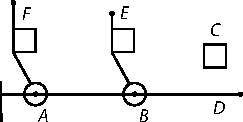
\includegraphics[width=0.35\textwidth]{gesamttex/edit_VIII,3/images/LH_37_05_001_d5.pdf}}%
  \vspace{1.0em}
  \centerline{\hspace*{78,0mm}\lbrack\textit{Fig.~5}\rbrack}%
  \label{LH_37_05_001r_Fig.5}%
%  \vspace{1.5em}%
%  \newpage%
%
%  \newpage% 
  \vspace{1.5em}%	% Diagramm Fig.~6
  \centerline{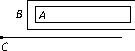
\includegraphics[width=0.30\textwidth]{gesamttex/edit_VIII,3/images/LH_37_05_001_d6.pdf}}% \hspace*{-85mm}
  \vspace{0.0em}
  \centerline{\lbrack\textit{Fig.~6}\rbrack}% \hspace*{-85mm}
  \label{LH_37_05_001r_Fig.6}%
  %\vspace{1.5em}%
  \newpage%
%
%
\pstart
\noindent  tantum circa
%
\edtext{\lbrack\textit{B}\rbrack,}{\lemma{%
\textit{E}}\Bfootnote{%
\textit{L~ändert Hrsg.}}}
%
immoto manente \textit{AB}.
Si vero tam uni quam alteri sit aequalis,
sequitur tamen solum fore motum\protect\index{Sachverzeichnis}{motus baculi}
\edlabel{LH_37_05_001r_demotu_kjdfgvk-1}circa \textit{B}.
%
\edtext{}{%
{\xxref{LH_37_05_001r_demotu_kjdfgvk-1}{LH_37_05_001r_demotu_kjdfgvk-2}}%
{\lemma{circa \textit{B}.}\Bfootnote{%
\textit{(1)}~Ex his positis sequitur etiam quid de funis rupti
\textit{(2)}~Sed quid \lbrack...\rbrack\ parte \textit{B} trahas,
\textbar~et esse quasi utrobique trahatur, \textit{erg.}~%
\textbar\ itaque cedetur \lbrack...\rbrack\ cessurum esse.
\textit{(a)}~Et hoc experiri
\textit{(b)}~Ex his \lbrack...\rbrack\ rumpi debeant,%
~\textit{L}}}}%
\pend%
% \newpage%
%
\pstart%
Sed quid si tractio\protect\index{Sachverzeichnis}{tractio}
sit in linea recta
ut si sit \textit{A} super \textit{B},
et \textit{B} ipsum super \textit{C} immobili,
et connectantur \textit{A} et \textit{B},
item \textit{B} et \textit{C} ope Elaterii;%
\protect\index{Sachverzeichnis}{elaterium connectens}
quaeritur si trahas quid futurum sit,
videtur nihil interesse
utrum a parte \textit{A} an a parte \textit{B} trahas,
et esse quasi utrobique trahatur,
itaque cedetur utrobique si aequales sunt.
Sin inaequales
videtur tantum inferius cessurum esse.
\pend
\pstart%
Ex his definiri posse videtur,
% \edlabel{LH_37_05_001r_demotu4}
quo loco fila%
\protect\index{Sachverzeichnis}{filum}\protect\index{Sachverzeichnis}{ruptura fili}
rumpi debeant,%
\edlabel{LH_37_05_001r_demotu_kjdfgvk-2}
nempe in debiliore,
itaque non miror
si cum rem experirer
variis locis fila sunt rupta,%
\protect\index{Sachverzeichnis}{filum}\protect\index{Sachverzeichnis}{ruptura fili}
sed redit difficultas,\protect\index{Sachverzeichnis}{difficultas}
quia hoc posito idem
%
\edtext{\lbrack ut\rbrack}{%
\lemma{et}\Bfootnote{%
\textit{L~ändert Hrsg.}}}
%
\edtext{supra}{%
\lemma{supra}\Cfootnote{%
S.~\refpassage{LH_37_05_001r_deduabustabulis_hgx-1}{LH_37_05_001r_deduabustabulis_hgx-2}.}}
%
de duobus tabulis%
\protect\index{Sachverzeichnis}{tabula plana}\protect\index{Sachverzeichnis}{tabulae compositae}
esset dicendum.
Si rem filis\protect\index{Sachverzeichnis}{filum} experiare,
omnibus paribus ruptura\protect\index{Sachverzeichnis}{ruptura fili}
fiet circa nodum\protect\index{Sachverzeichnis}{nodus} infimum
ex quo pondus pendet,\protect\index{Sachverzeichnis}{pondus pendens}
vel si duo sint fila,\protect\index{Sachverzeichnis}{filum}
et inferius fortius,
ruptura\protect\index{Sachverzeichnis}{ruptura fili} fiet in eorum confinio.
Si
%
\edtext{tamen locus aliquis}{%
\lemma{tamen}\Bfootnote{%
\textit{(1)}~unum
\textit{(2)}~locus
\textit{(a)}~aliquid
\textit{(b)}~aliquis%
~\textit{L}}}
%
sit valde debilis,
ibi fit ruptura,\protect\index{Sachverzeichnis}{ruptura fili}
salvo
%
superiore principio,\protect\index{Sachverzeichnis}{principium}
% \edtext{}{%
% \lemma{superiore principio}\Cfootnote{% ?????}}
%
quod superatur
%
\lbrack1~v\textsuperscript{o}\rbrack\ % % % %  Blatt 1v
%
proximum quando superari potest.
Hic enim etsi proximum
%
\edtext{fortius}{%
\lemma{fortius}\Bfootnote{%
\textit{erg.~L}}}
%
quoque superari possit,
superatur
%
\edtext{tamen debilius}{%
\lemma{tamen}\Bfootnote{%
\textit{(1)}~remotius
\textit{(2)}~remot
\textit{(3)}~debilius%
~\textit{L}}}
%
licet remotius.
Quia proximum hoc initio non potest superari,
%
% \edtext{}{%
% \lemma{initio}\Bfootnote{%
% \textit{(1)}~insuperabil
% \textit{(2)}~non potest superari,%
% ~\textit{L}}}
%
nec nisi
%
\edtext{paulatim fila\protect\index{Sachverzeichnis}{filum}}{%
\lemma{paulatim}\Bfootnote{%
\textit{(1)}~in fili
\textit{(2)}~fila%
~\textit{L}}}
%
fiunt capacia rupturae.\protect\index{Sachverzeichnis}{ruptura fili}
Hinc cum debilius prius fiat superabile,
ibi quoque prius fit ruptura.\protect\index{Sachverzeichnis}{ruptura fili}
Sed cum omnia sunt paria\lbrack,\rbrack\
ruptura\protect\index{Sachverzeichnis}{ruptura fili} fit in loco propiore. 
\pend%
%
\pstart%
Experimenta ergo\protect\index{Sachverzeichnis}{experimentum nulli exceptioni subjacens}
quae nulli exceptioni subjacent,
et rem clare ostendunt
sunt mechanica\protect\index{Sachverzeichnis}{experimentum mechanicum}
ponderibus\protect\index{Sachverzeichnis}{pondus adhibitum}
sive Elateriis connectentibus\protect\index{Sachverzeichnis}{elaterium connectens} adhibitis.
Quae si favent sententiae\protect\index{Sachverzeichnis}{sententia} meae,
%
% \edtext{}{%
% \lemma{sententiae meae}\Cfootnote{TILGEN ???}}
%
hinc singulari constat exemplo,\protect\index{Sachverzeichnis}{exemplum singulare}
quantum intersit inter motum absolutum,\protect\index{Sachverzeichnis}{motus absolutus}
et respectivum.\protect\index{Sachverzeichnis}{motus respectivus}
\pend%
% \newpage%
%
\pstart%
Idem ut confirmetur,
hoc utamur experimento\lbrack:\rbrack\
in globum unum pendulum\protect\index{Sachverzeichnis}{globus pendulus}
%
\edtext{quiescentem}{%
\lemma{quiescentem}\Bfootnote{%
\textit{erg.~L}}}
%
alius argillaceus\protect\index{Sachverzeichnis}{globus argillaceus} demittatur aequalis,
si motus respectivus\protect\index{Sachverzeichnis}{motus respectivus}
hic nihil differt ab absoluto,\protect\index{Sachverzeichnis}{motus absolutus}
idem erit eventus\protect\index{Sachverzeichnis}{eventus}
qui ambis in se invicem incurrentibus,
nimirum quiescent ambo simul.
\pend%
%
\pstart%
Casus\protect\index{Sachverzeichnis}{casus inanis}%
\edlabel{LH_37_05_001v_casusinanis_rltn-1}
ut duo corpora dura\protect\index{Sachverzeichnis}{corpus durum}
in vacuo\protect\index{Sachverzeichnis}{vacuum} concurrant,%
\protect\index{Sachverzeichnis}{concursus in vacuo}
est inanis,
%
\edtext{atque alienus a natura rerum.%
\protect\index{Sachverzeichnis}{casus alienus a natura rerum}}{%
\lemma{atque}\Bfootnote{%
\textit{(1)}~impossibilis
\textit{(2)}~alienus a natura rerum.%
~\textit{L}}}
%
Nam semper in omni incursu\protect\index{Sachverzeichnis}{incursus}
cessio\protect\index{Sachverzeichnis}{cessio} est
et restitutio\protect\index{Sachverzeichnis}{restitutio}
etsi ea saepe a nobis non sentiantur,
cum spongiosa corpora\protect\index{Sachverzeichnis}{corpus spongiosum} sunt,
et motus per partes dispergitur.%
\protect\index{Sachverzeichnis}{motus per partes dispersus}
Quoties vero non dispergitur,
sed integer\protect\index{Sachverzeichnis}{motus integer} apparet
%
\edtext{motus\lbrack,\rbrack\
apparet praeclarum illud principium,%
\protect\index{Sachverzeichnis}{principium naturae}}{%
\lemma{motus}\Bfootnote{%
\textit{(1)}~verissima est
\textit{(2)}~apparet praeclarum illud
\textit{(a)}~naturae p
\textit{(b)}~Metaph
\textit{(c)}~principium,%
~\textit{L}}}
%
Conatum naturae\protect\index{Sachverzeichnis}{conatus naturae}\protect\index{Sachverzeichnis}{natura}
semper irresistibilem esse.%
\protect\index{Sachverzeichnis}{conatus irresistibilis}
Semper centrum gravitatis mobilium%
\protect\index{Sachverzeichnis}{centrum gravitatis mobilis}
in eadem recta procedet.%
\edlabel{LH_37_05_001v_casusinanis_rltn-2}
\pend%
%
\pstart%
\edtext{Quoties major}{%
\lemma{Quoties}\Bfootnote{%
\hspace{-0,5mm}\textbar~deinde \textit{streicht}~%
\textbar\ major%
~\textit{L}}}
%
est firmitas corporis\protect\index{Sachverzeichnis}{firmitas corporis}
quam ictus,\protect\index{Sachverzeichnis}{ictus}
totum propellitur.
Si quis totam rerum machinam\protect\index{Sachverzeichnis}{machina rerum} tamen intueretur,
videret corpus hoc\protect\index{Sachverzeichnis}{corpus cedens}
quod cedit totum\lbrack,\rbrack\
considerandum ut alterjus partem
in quo et restitutio est,\protect\index{Sachverzeichnis}{restitutio insensibilis}
sed quae in nostro hoc corpore non est sensibilis,
cum per tot alia distribuatur.\protect\index{Sachverzeichnis}{restitutio distributa}
\pend%
\count\Bfootins=1200
\count\Afootins=1200
\count\Cfootins=1200
%
%
% % % %  ENDE des Stücks auf Blatt 1v
%